\documentclass{article}
\usepackage{tikz}
\begin{document}

\begin{figure}[h!]
    \centering
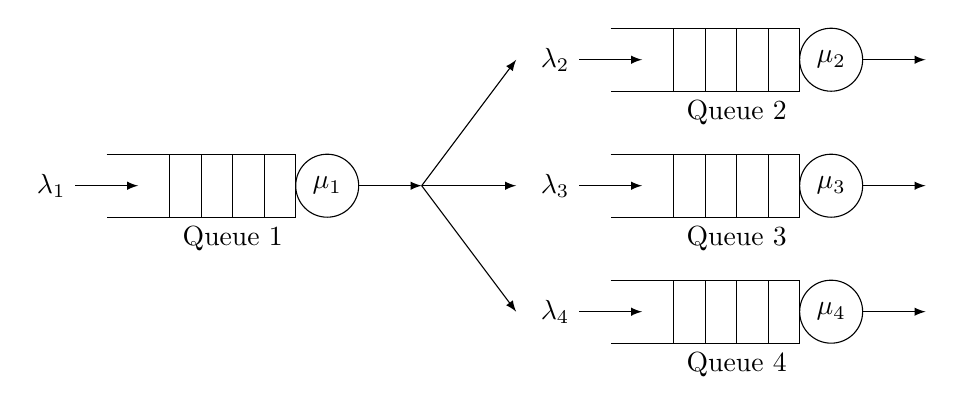
\begin{tikzpicture}[>=latex,scale=0.8]
    \foreach \x/\y/\n in {0/0/1,8/2/2,8/0/3,8/-2/4}
    {
          \pgfmathsetmacro{\r}{0.5} % radius of the circles
          \pgfmathsetmacro{\l}{3} % total length of the queue
          %draw the rectangle of the queue
          \draw (\x-\r-\l,\y+\r) -- ++(\l,0) -- ++(0,-2*\r) -- ++(-\l,0);
          % vertical bars of the queue
          \foreach \i in {1,...,4}
            \draw (\x-\r-\i*0.5,\y+\r) -- +(0,-2*\r);
          
          % the server
          \draw (\x,\y) circle (\r);
          %arrow with arriving rate
          \draw[<-] (\x-\l,\y) -- +(-2*\r,0) node[left] {$\lambda_\n$};
          %arrow for departure
          \draw[->] (\x+\r,\y) -- +(2*\r,0);
          % service rate
          \node at (\x,\y) {$\mu_\n$};
          % name of the queue
          \node [below] at (\x-\l/2,\y-\r) {Queue \n};
    };
    \draw[->] (1.5,0) -- (3,2);
    \draw[->] (1.5,0) -- (3,0);
    \draw[->] (1.5,0) -- (3,-2);
\end{tikzpicture}
 \caption{Queue Network}\label{fig:queueNetwork}
\end{figure}

\end{document} 
